\documentclass{report}

% Language setting
% Replace `english' with e.g. `spanish' to change the document language
\usepackage[english]{babel}

% Set page size and margins
% Replace `letterpaper' with `a4paper' for UK/EU standard size
\usepackage[letterpaper,top=2cm,bottom=2cm,left=3cm,right=3cm,marginparwidth=1.75cm]{geometry}

% Useful packages
\usepackage{amsmath}
\usepackage{graphicx}
\usepackage{float}
\usepackage{subcaption}
\usepackage[colorlinks=true, allcolors=blue]{hyperref}

\newtheorem{definition}{Definition}[section]

\title{Protein Structures}
\author{Vinay Kakkar}

\begin{document}
\maketitle

\tableofcontents

\begin{abstract}

Three-dimensional structures are created from sequences of amino acids in polypeptide chains folds that are generated from linear chains. The folded domains can serve as modules for building up large assemblies such as a muscle fiber but more importantly, they can provide specific catalytic or binding sites, as found in enzymes or proteins. We look at the foundations of a protein such as the building blocks. Using technologies in order to read these sequences of amino acids into information that helps determine what the function of the structure will have. Using our knowledge of protein structures and bioinformatics, we can achieve the goal of predicting functions of proteins from a large set of data provided by experiments such as, DNA microarray technology and Two-dimensional Gel electrophoresis or Chromatography. With new technologies such as AlphaFold, we can even predict the 3D structure of a Protein using the amino acid sequence alone.

\end{abstract}

\renewcommand\thesection{\arabic{section}}

\section{Introduction}
Amino acids are molecules that when combined together it forms proteins. All of the 20 amino acids, see table~\ref{Amino acids} have in common a central carbon atom which are attached a hydrogen atom, an amino group and a carboxyl group. What distinguishes one amino acid from another is the side chain attached to the central carbon atom through its fourth valence~\cite{branden_introduction_1998}.

\begin{table}[h!]
    \begin{center}
    \label{tab:Amino acids}
        \begin{tabular}{l|c|r}
        Amino acid & Three-letter code & One-letter code\\
        \hline
        \\
        Glycine & Gly & G\\
        Alanine & Ala & A\\
        Valine & Val & V\\
        Leucine & Leu & L\\
        Isoleucine & Ile & I\\
        Proline & Pro & P\\
        Phenylalanine & Phe & F\\
        Methionine & Met & M\\
        Tryptophan & Trp & W\\
        Cysteine & Cys & C\\
        \\
        \hline
        \\
        Asparagine & Asn & N\\
        Glutamine & Gln & Q\\
        Serine & Ser & S\\
        Threonine & Thr & T\\
        Tyrosine & Tyr & Y\\
        \\
        \hline
        \\
        Aspartic acid & Asp & D\\
        Glutamic acid & Glu & E\\
        \\
        \hline
        \\
        Histidine & His & H\\
        Lysine & Lys & K\\
        Arginine & Arg & R\\
        \end{tabular}
        \caption{\label{Amino acids}The 20 amino acids. The amino acid name, the three-letter code, and the one-letter code are given. The Amino acids are split up into Nonpolar, Polar, Acidic and Basic respectfully}
    \end{center}
\end{table}

Proteins are responsible of catalysing most the chemical reactions in cells. They can function as enzymes catalysing a wide variety of reactions important for life and thus also important for the structure of living systems such as proteins involved in the cytoskeleton. The size of protein can vary ~\cite{zvelebil_understanding_2008}.

\begin{definition}[Catalysing]
    Catalysing is to make a chemical reaction happen or happen more quickly by acting as a catalyst.
\end{definition}

\begin{definition}[Cytoskeleton]
    A dynamic network of interlinking protein filaments present in the cytoplasm of all cells~\cite{zvelebil_understanding_2008}. 
\end{definition}

We can analyse a DNA sequence of a gene to retrieve the amino acid sequence of the protein product, using the fact that protiens are a built up off amino acids.Leaving a position where we can help deduce the likely properties of unknown proteins, whilst at the same time including their functions and structures. Knowing the relationship between a proteins structure and its function provides a better understanding of how the protein works ti better understand this we can conduct experiments to explore how modifying the structure will affect the function. The use of bioinformatics aids this process whilst also providing computer modelling for these interactions~\cite{zvelebil_understanding_2008}.

\section{Protein Structure}

\subsection{Primary, Secondary, Tertiary and Quaternary Structure}

\subsubsection{Primary Structure}

The primary structure of a peptide or protein is the linear sequence of its amino acids. It is read and written from the amino-terminal to the carboxyl-terminal end. Where each amino acid is connected to the next by a peptide bond. Primary strucutre sequence it can interact with one another to form secondary structures~\cite{noauthor_levels_nodate}.

\subsubsection{Secondary Structure}

The secondary structure refers to the local arrangement of a peptide chain. Where several common secondary structures have been identified in proteins~\cite{noauthor_levels_nodate}.

\subsubsection{Tertiary Structure}

Tertiary structure is a three-dimensional structure of a protein the formation is built up of bonds and interactions that serve to change the shape of the overall protein. Finaly the folding that we end up with for a given polypeptide is the tertiary structure~\cite{godbey_chapter_2022}.

\subsubsection{Quaternary Structure}

Quaternary structure of a protein is the built up of several protein chains/subunits. Each of the subunits has its own primary, secondary, and tertiary structure. The subunits are held together by hydrogen bonds and van der Waals forces between nonpolar side chains~\cite{ouellette_14_2015}.

\begin{definition}[Van Der Waals]
    A relatively weak electric force that attract neutral molecules that collide with or pass very close to each other~\cite{noauthor_210_2018}.
\end{definition}

\begin{table}[h!]
    \begin{center}
    \label{tab:Quanternanry Protiens}
        \begin{tabular}{l|c|r}
            \hline
            Protein & Number of Subunits & Function\\
            \hline
            Alcohol dehydrogenase & 4 & Enzymatic reaction in fermentation\\ 
            \hline
            Aldolase & 4 & Enzymatic reaction in glycolysis\\
            \hline
            Fumarase & 4 & Enzymatic reaction in citric acid cycle \\
            \hline
            Hemoglobin & 14 & Oxygen transport in blood\\
            \hline
            Insulin & 2 & 6344\\
            \hline
        \end{tabular}
        \caption{\label{Quanternanry Protiens}Examples of Proteins Having Quaternary Structure~\cite{ouellette_14_2015}.}
    \end{center}
\end{table}


\begin{figure}[H]
    \centering
    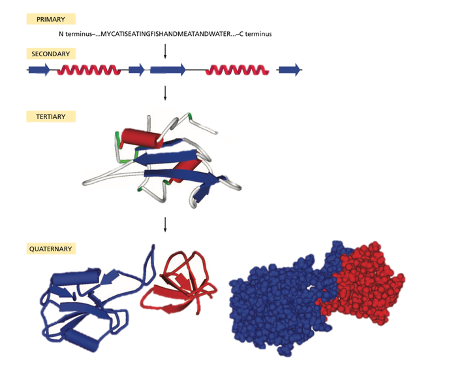
\includegraphics[width=0.5\textwidth]{Protein Structure.png}
    \caption{\label{fig:levels of protein structure.}From the sequence alone, the primary structure to secondary structure, to tertiary structure(3D), to finally quaternary structure found when several tertiary structures form a multisubunit complex~\cite{zvelebil_understanding_2008}.}
\end{figure}

\subsubsection{Considering Protein structure on several different levels}

The fold of the protein plays part in determining the way the protein will function, and also whether it will function correctly so it is important to understand these folds. Which we can use to help us for example predicting the fold of a protein from its sequence. Looking at Protein structures on different levels we need to consider the analysis of protein structure by experimental techniques such as X-ray crystallography, nuclear magnetic resonance and RNAseq which show that proteins adopt distinct structural elements~\cite{zvelebil_understanding_2008}.

\subsubsection{Amino Acids}

When looking at a primary structure of a protein the sequence of amino acids will build up the linear protein chain. This linear chain is often called a polypeptide chain~\cite{zvelebil_understanding_2008}.

Amino acids are different to each other due to their side chains and due to this the functional properties various different proteins are different. Each type of amino acid has specific chemical physical properties determined by the structure and chemical properties of its side chain. They can, however, be classified into overlapping groups that share some common physical and chemical properties~\cite{zvelebil_understanding_2008}.


\begin{figure}[H]
    \centering
    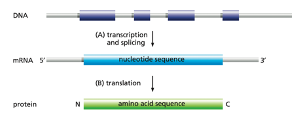
\includegraphics[width=0.5\textwidth]{Transcription and translation.png}
    \caption{\label{fig:Transcription and translation}The relation of DNA coding-strand sequence to mRNA sequence to protein sequence. The exons (purple boxes) of the DNA are transcribed into mRNA which, using other molecules directs the protein sequence~\cite{zvelebil_understanding_2008}.}
\end{figure}

\subsubsection{Bioinformatic Difficulties with Predictions on Proteins}

It is difficult to define the percise ends of the helices(Secondary structure of proteins is made up of a-helices and b-strands) for structures found in globular proteins that are not perfectly regular. Making it one step more difficult when trying to predict these structures~\cite{zvelebil_understanding_2008}.

To Note:
\begin{itemize}
    \item Several different types of b-sheet are found in protein structures.
    \item Turns, hairpins, and loops connect helices and strands. 
    \item Any chain between two regular structures is referred to as a loop.
    \item Mostly a loop will contain a turn (or even several).
\end{itemize} 

In antibody recognition, immunoglobulins employ loops at the edge of a b-sheet. All immunoglobulin structures with the same overall chain fold, but it is the difference at these loops that results in different results. Loops take up one of a limited number of structures called canonical forms. This type of classification is another reason why trying to predict both the structure and function of the protein is difficult~\cite{zvelebil_understanding_2008}.

\begin{definition}[Immunoglobulin]
    Immunoglobulins are heterodimeric proteins composed of two heavy and two light chains. Types of white blood cells that helps the body fight infection~\cite{schroeder_structure_2010}.
\end{definition}

\subsection{Compact Structures}

\subsubsection{Protein Folds}

Protein chains by themselfes no major function. Only does so once the chain has folded up into a tertiary or quaternary structure  ~\cite{zvelebil_understanding_2008}. 

For example:

Proteins enzymes bind to other molecules (ligands) and catalyze their biochemical reactions, or they can influence proteins activity, or regulate gene expression by binding to DNA. In other cases proteins have a purely structural function for example, making up the fabric of the cell. Or for example, proteins acting as chemical messengers are released, from cells which, influence the behavior of other cells by acting on another class of proteins, known as receptors~\cite{zvelebil_understanding_2008}.

The tertiary structure is defined by the path of its polypeptide chain in the tertiary structure of a protein where each domain folds independently of the others~\cite{zvelebil_understanding_2008}.

\subsubsection{Bioinformatics with Protein Folds}

Bioinformatics more intrested in the sequences and structures of different domains over whole proteins where a domian can vary from 50 to around 350 amino acids in length ~\cite{zvelebil_understanding_2008}.

There is a limited number of ways secondary structures fold into domains.

For example we have had proteins that seem to be completely unrelated in terms of sequence are found to have the same fold giving the idea that there may be finite number of folds in nature.

As proteins can fold into a similar structure even if their sequences are not very similar means that we can use bioinformatics tools to model structures of various proteins on similar folds~\cite{zvelebil_understanding_2008}.

\section{Large Scale Experssion}

Gene expression begins when genes are transcribed into messenger RNAs, which are then translated to produce proteins. 

Total gene expression in cultured cells or a tissue sample can be detected in three main ways:

\begin{enumerate}
    \item DNA microarray technology.
    \item Two-dimensional Gel electrophoresis or Chromatography.
    \item RNAseq
\end{enumerate}

With the first two cases they produce enormous amounts of raw data~\cite{zvelebil_understanding_2008} due to this, many proteins currently evade high-resolution structure determination. Structural mass spectrometry is a powerful approach that better then the first two methods mentioned above, by having nearly a unlimited size constraint, and speed. Although the data provided by mass spectrometry is vauge for full high-resolution structure elucidation, structural mass spectrometry can be used to examine the size, solvent accessibility, and topography of proteins~\cite{limpikirati_covalent_2018}~\cite{liu_mass_2020}.  Many mass spectrometry techniques exist that can elucidate elements of protein tertiary and quaternary structure~\cite{biehn_protein_2022}.

We can have computational methods that aid experimental technique with the goal to elucidate protein structures~\cite{seffernick_hybrid_2020}~\cite{leman_macromolecular_2020}. Software packages can be used to combine data with advanced structure sampling and scoring techniques. Computational tools for protein structure modeling, include the Rosetta software suite~\cite{leman_macromolecular_2020}~\cite{alford_rosetta_2017}, I-TASSER~\cite{yang_i-tasser_2015}, Phyre2~\cite{kelley_phyre2_2015}, Integrative Modeling Platform~\cite{russel_putting_2012}, HADDOCK~\cite{dominguez_haddock_2003}, and MODELLER~\cite{eswar_comparative_2006}~\cite{biehn_protein_2022}.

\subsection{Large Scale Gene Expression}

Genome DNA microarray experiments produce large amount of data can be computationaly heavy on where methods can yield alternative conclusions from inceasing the computational effort.

The goal of these experiments is to determine biological or functional meaning from the lists of genes, either by:

\begin{enumerate}
    \item Identify critical genes that are responsible for a biological effect.
    \item Find patterns within the genes that point to an underlying biological process.
\end{enumerate}
\cite{zvelebil_understanding_2008}

\begin{figure}[H]
    \centering
    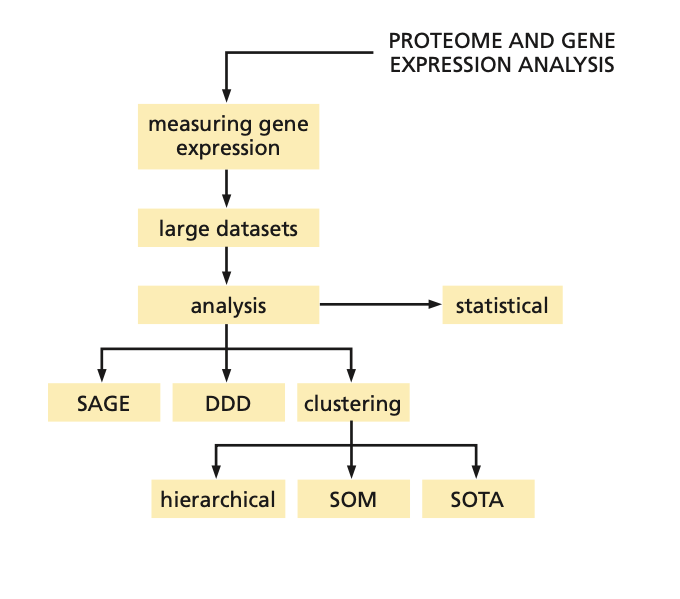
\includegraphics[width=0.5\textwidth]{Gene Expresion.png}
    \caption{\label{fig:Gene Expression}Describing Common experimental aspects of gene expression and of the analysis of the resulting data~\cite{zvelebil_understanding_2008}.}
\end{figure}

\subsubsection{Serial analysis of gene expression}

Serial analysis of gene expression is the alternative compared to microarrays when trying to investigate patterns of gene expression.

\begin{figure}[!h]
    \centering
    \begin{subfigure}[t]{.45\textwidth}
        \centering
        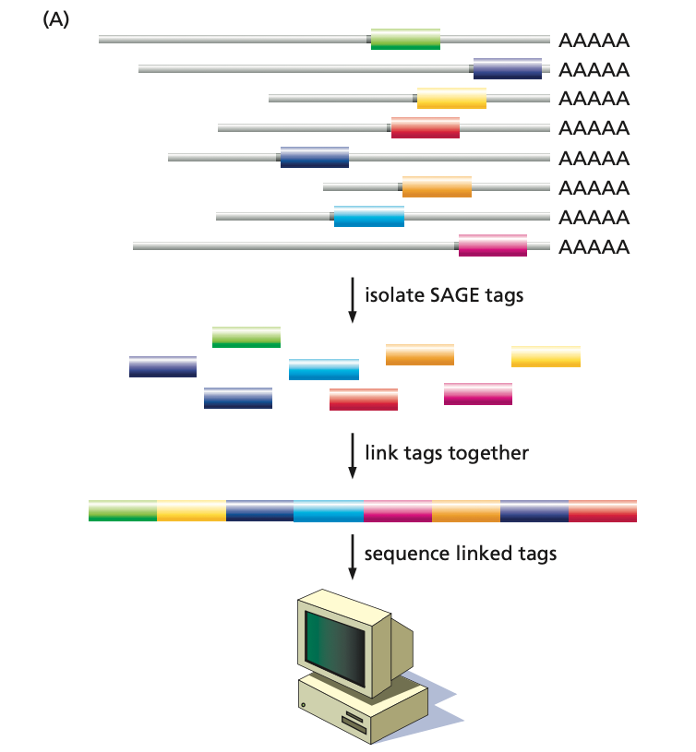
\includegraphics[width=0.9\textwidth]{SAGE1.png}
        \caption{}
        \label{fig:SAGE1} 
    \end{subfigure}
    \begin{subfigure}[t]{.45\textwidth}
       \centering
       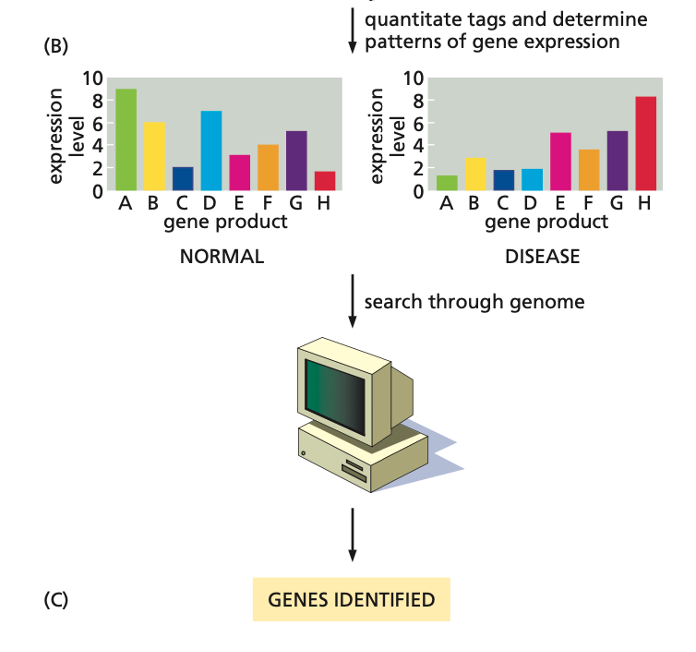
\includegraphics[width=0.9\textwidth]{SAGE2.png}
       \caption{}
       \label{fig:SAGE2}
    \end{subfigure}
    \caption{\emph{An outline of the SAGE method for comparing levels of gene expression. (A) Short sequence tags. The sequence tags are isolated and are linked together to produce long DNA molecules that can be cloned and sequenced. (B) Once sequenced, each tag can be calculated, resulting in a value that gives the expression level of the corresponding transcript~\cite{zvelebil_understanding_2008}.}}
    \label{fig:SAGE}
\end{figure}


A short sequence contains enough information to uniquely identify a gene. The sequence tags from the total cellular RNA can be linked together to form long DNA molecules. The total number of times a particular tag is observed the concatemers approximates the expression level of the corresponding gene. The data produced by SAGE include a list of the tags with their corresponding counts, providing a digital output of cellular gene expression.  Which allow the user to specify which organ is to be investigated. Libraries consisting of gene lists organized by the various types of tissues or cell lines are provided for further choice. The output from SAGE provides the SAGE tag, the UniGene ID, the gene description, and color and letter coded differences in expression levels~\cite{zvelebil_understanding_2008}.

\subsubsection{Clustered gene expression data}

Clustered pattern data obtained from gene expression microarrays/genome bioinformatics can be used as a tool to identify new transcription factors or other cell-regulatory proteins. 

The clustered genes/proteins can be analyzed. Leading to a vast collection of data from many gene/protein expression expeniments being available on the Web~\cite{zvelebil_understanding_2008}.

\subsection{Large Scale Protein Expression}

\begin{figure}[H]
    \centering
    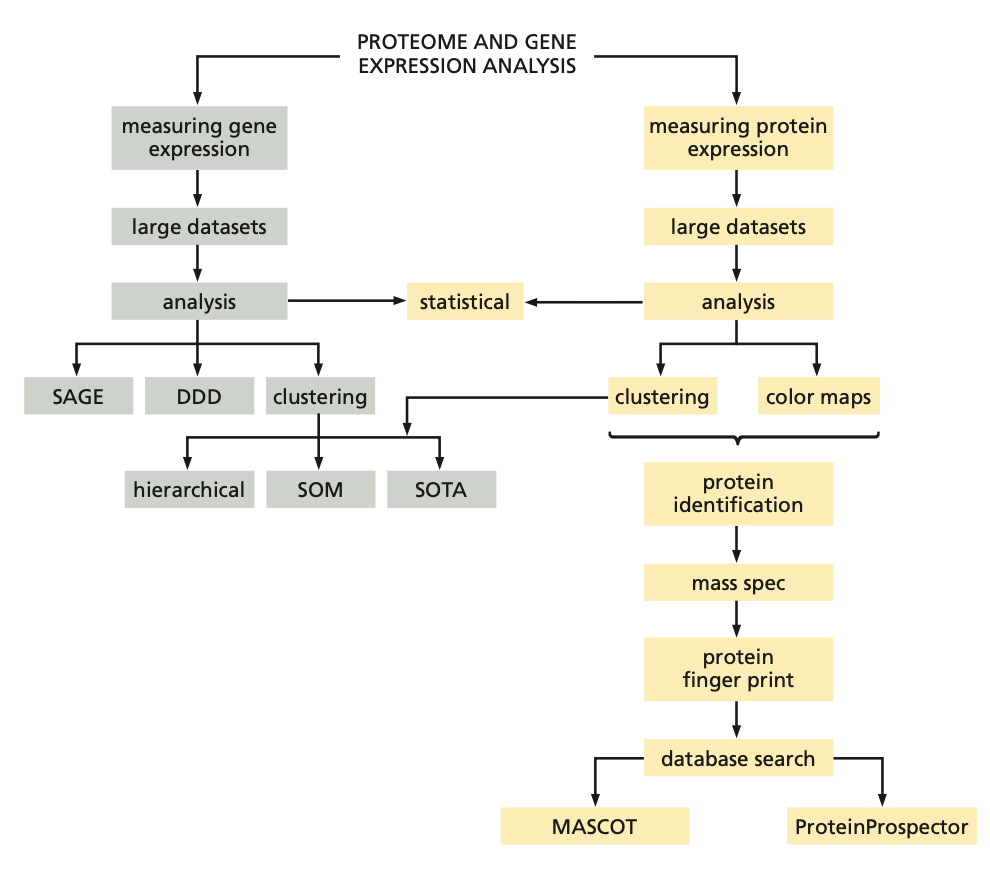
\includegraphics[width=0.5\textwidth]{Overlaping.png}
    \caption{\label{fig:Overlaping}Describing some experimental aspects of protein expression and of the analysis of the resulting data.~\cite{zvelebil_understanding_2008}.}
\end{figure}

For functional protein, mRNAs need to be translated, whilst the protein products can change which influence their function. For this reason we can measure and anlayse different proteins. 

There is more proteins than there are genes in a genome. Transcripts can be spliced in various ways to give different mRNAs, providing different protein products, from the same gene. However, proteins that can be modified after translation giving more different protien products.

Protien expressions can vary in a organism depending on the origin and it will also differ between the separate stages of an organism’s life cycle and under different environmental conditions. 

\begin{definition}[proteome]
    The proteome refers to all the proteins that make up an organism at a specific point in time and under specific conditions.
\end{definition}

It is important to know how protein expression is affected in order to understand how an organism or a cell functions~\cite{zvelebil_understanding_2008}.

\subsection{RNAseq}

Transcriptome is important for revealing the molecular constituents of cells and tissues, interpreting the functional aspects of the genome and, also for understanding development and disease~\cite{wang_rna-seq_2009}.

Many methods deduce and quantify the transcriptome, including hybridizationor sequence-based approaches. For example hybridization-based approaches which involve incubating fluorescently labelled cDNA with microarrays or commercial high-density oligo microarrays~\cite{wang_rna-seq_2009}.

However, these methods have several limitations, such as: 
\begin{itemize}
    \item Dreliance upon existing knowledge about genome sequence.
    \item Limited dynamic range of detection owing to both background.
    \item High background levels owing to cross-hybridization~\cite{okoniewski_hybridization_2006}~\cite{royce_toward_2007}.
    \item saturation of signals.
\end{itemize}

\begin{definition}[transcriptome]
    The transcriptome is the complete set of transcripts in a cell, and their quantity, for a specific developmental stage or physiological condition. 
\end{definition}

Sequence-based approaches directly determine the cDNA sequence such as, Tag-based methods which include SAGE, CAGE~\cite{kodzius_cage_2006}, MPSS~\cite{reinartz_massively_2002}.

Each approach are high throughput and can provide precise, gene expression levels. However, significant portion of the short tags can not be uniquely mapped to the reference genome~\cite{wang_rna-seq_2009}.

RNA-Seq RNA sequencing, has clear advantages over existing approaches it uses deepsequencing technologies where a population of RNA is converted to a library of cDNA fragments with adaptors attached to one or both ends. Each molecule is then sequenced in a high-throughput manner to obtain short sequences from one or both ends~\cite{wang_rna-seq_2009}.

\begin{figure}[H]
    \centering
    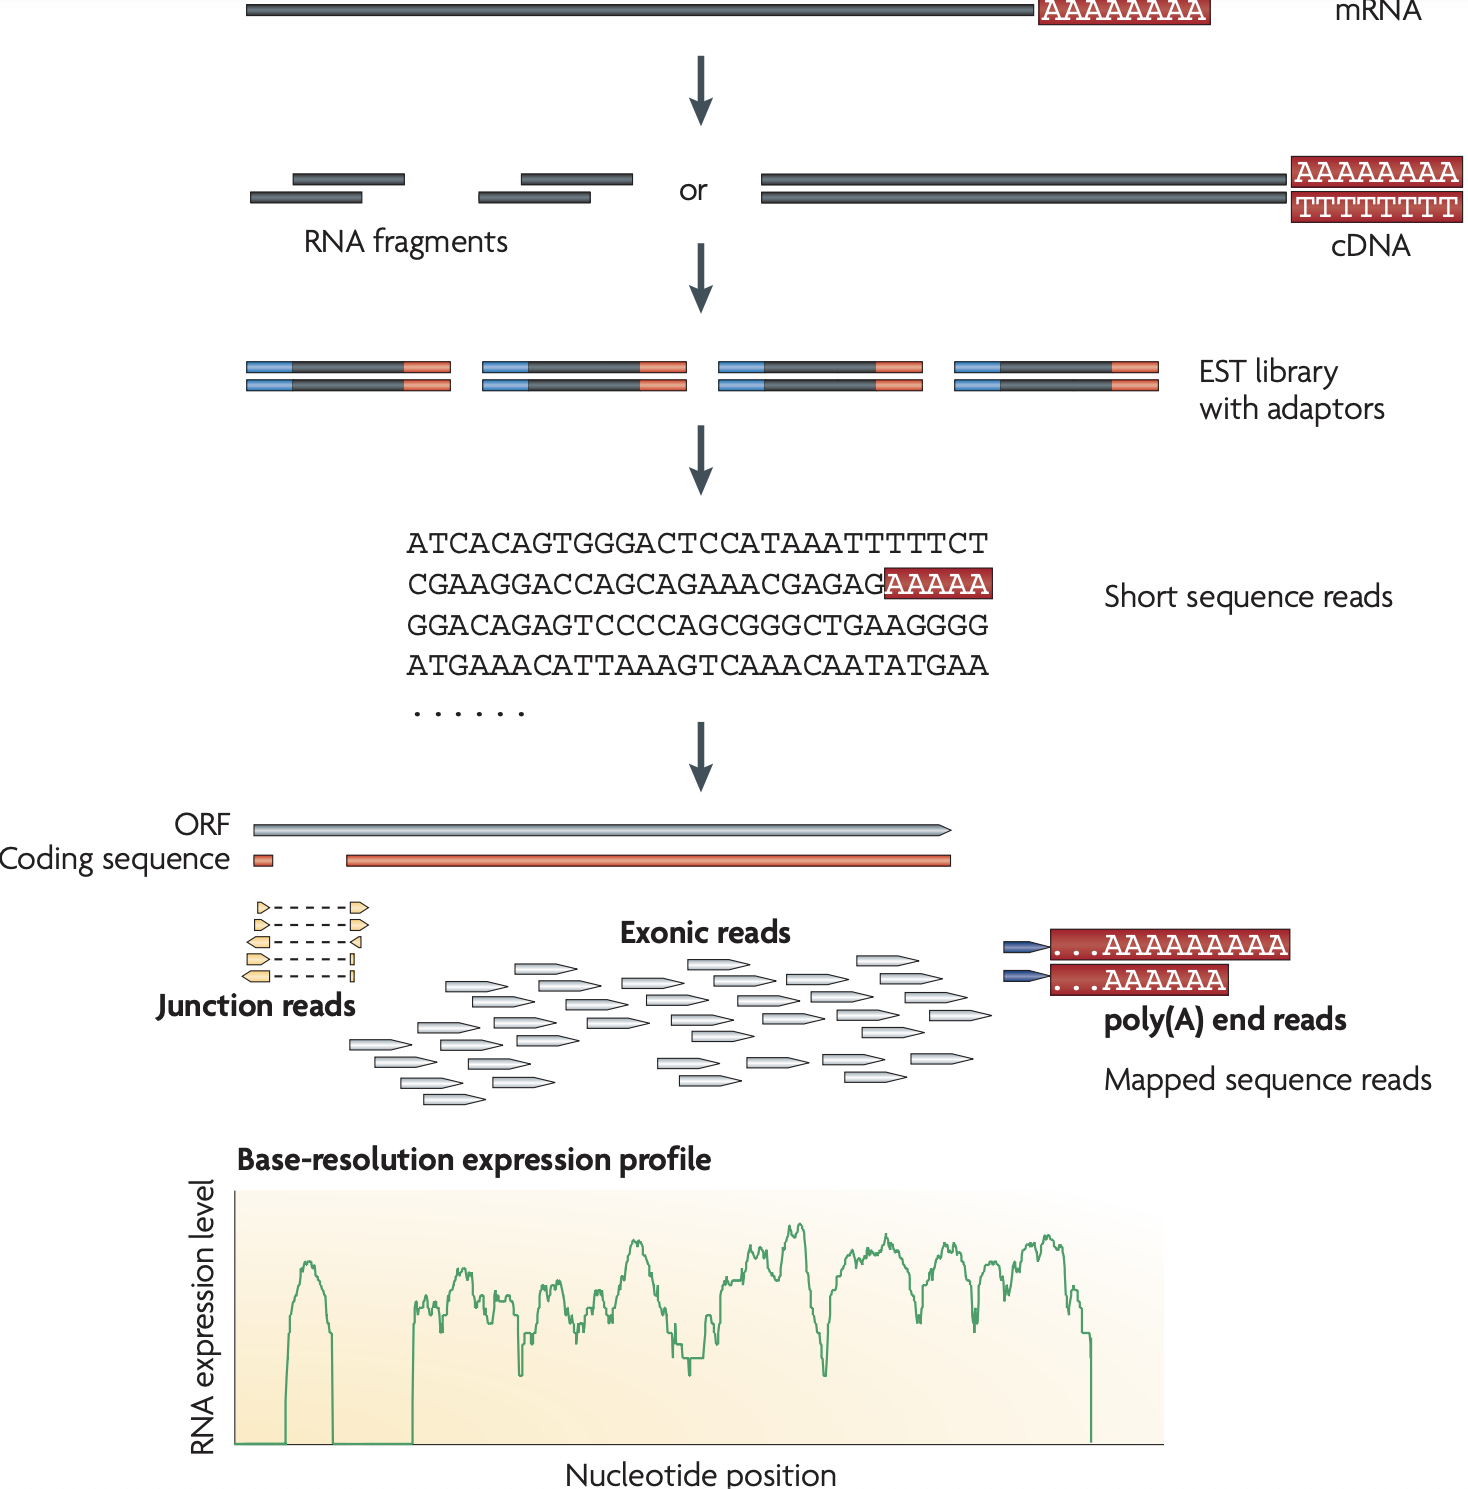
\includegraphics[width=0.5\textwidth]{RNAseq.png}
    \caption{\label{fig:RNAseq}A typical RnA-seq experiment. RNAs are first converted into a library of cDNA fragments through either RNA fragmentation or DNA fragmentation. Sequencing adaptors are subsequently added to each cDNA fragment and a short sequence is obtained from each cDNA using high-throughput sequencing technology. The resulting sequence reads are aligned with the reference genome or transcriptome.}
\end{figure}


\section{Alpha Fold}

AlphaFolds goal is to  predict the 3D coordinates of all heavy atoms for a given protein using the primary amino acid sequence and aligned sequences of homologues as inputs~\cite{jumper_highly_2021}.

Mutations in proteins can lead to misfolding which is often associated with disease states, for example, Alzheimer’s and Parkinson’s which is one of the chanllanges for alphaFold~\cite{felix_brief_nodate}.

The output is a file containing the 3D coordinates for every non-hydrogen atom in the protein. whilst showing the confidence levels for every amino acid residue, providing the reliability of the predicted structure~\cite{felix_brief_nodate}.

\subsubsection{Bioinformatics with Alpha Fold}

Look for how alpha fold started
Find more about how alpha fold works
In July 2021, AlphaFold was developed by DeepMind, and was made available to
the public~\cite{tunyasuvunakool_highly_2021}. 

Where it tries to silve the issue of invariant protein structures that are under translations and rotations~\cite{baldi_principled_nodate}.

AlphaFold is trained on protein chains from the PDB using the input sequence to query databases of protein sequences to generate a multiple sequence alignment~\cite{jumper_highly_2021}. Although we still do no exactly know how a protein sequence fold and alphafold does not help in figureing this out but its impact will likely be in accelerating and improving production of new medications~\cite{nussinov_alphafold_2022}.


\subsection{AlphaFold 2}

The CASP14 was recently held which is a blind trial that critically assesses
techniques for protein structure prediction~\cite{david_alphafold_2022}, AlphaFold2 was entered and out-performed all comptetitors. 

Recently, RoseTTAFold was developed, trying to implement similar principles. Since then, other end-to-end structure predictors have emerged using different principles such as fast multiple sequence alignment processing in DMPFold218 and language model representations.\cite{bryant_improved_2022}.

We use the root mean square deviation, to calculate the similarity between two structures, AlphaFold models had a accuracy of 0.96 compared to 2.80 which was the second best score. AlphaFold models also had a high level of accuracy in predicting the position of residue side chains when the protein backbone prediction was accurate~\cite{david_alphafold_2022}~\cite{jumper_highly_2021}.


\section{Implication for Bioinformatics}

Bioinformatics concerns itself with the analysis of protein sequence to predict the structures, as well as its relationship to other proteins resulting in predicting the functionality.~\cite{zvelebil_understanding_2008}.

\bibliographystyle{alpha}
\bibliography{bibliography}


\end{document}